\songchapter{L}

%%%%%%%%%%%%%%%%%%%%%%%%%%%%%
\songsection{罗大佑}	\index{L!luodayou}

%%%%%%%%%%%%%%%%%%%
\subsection{未来的主人翁}

\begin{figure}[htp]
	\begin{center}
	  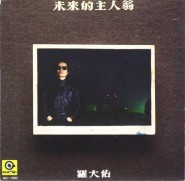
\includegraphics[scale = 0.80]{l/luodayou/weilaidezhurenweng}
% 	  \caption[labelInTOC]{未来的主人翁}
	  \label{fig:weilaidezhurenweng}
	\end{center}
\end{figure}

\begin{songs}{}
  \beginsong{未来的主人翁}[index={未来的主人翁}]
	你走过林立的高楼大厦穿过那些拥挤的人	\\
	望着一个现代化的都市泛起一片水银灯	\\
	突然想起了遥远的过去未曾实现的梦	\\
	曾经一度人们告诉你说你是未来的主人翁	\\
	\vspace{2ex}
	在人潮汹涌的十字路口每个人在痴痴地等	\\
	每个人的眼睛都望着那象征命运的红绿灯	\\
	在红橙黄绿的世界里你这未来的主人翁	\\
	在每一张陌生的面孔里寻找儿时的光荣	\\
	\vspace{2ex}
	每一个今天来到世界的婴孩	\\
	张大了眼睛摸索着一个真心的关怀	\\
	每一个来到世界的生命在期待	\\
	因为我们改变的世界将是他们的未来	\\
	\vspace{2ex}
	别以为我们的孩子们太小他们什么都不懂	\\
	我听到无言的抗议在他们悄悄的睡梦中	\\
	我们不要一个被科学游戏污染的天空	\\
	我们不要被你们发明变成电脑儿童	\\
	\vspace{2ex}
	每一个今天来到世界的婴孩	\\
	张大了眼睛摸索着一个真心的关怀	\\
	每一个来到世界的生命在期待	\\
	因为我们改变的世界将是他们的未来	\\
	\vspace{2ex}
	有一天孩子们会告诉他们后代你们要守规矩	\\
	格言象玩具风筝在风里飘来飘去	\\
	当未来的世界充满了一些陌生的旋律	\\
	你或许会想起现在这首古老的歌曲	\\
	\vspace{2ex}
	飘来飘去 \hspace{5mm} 就这么飘来飘去	\\
	飘来飘去 \hspace{5mm} 就这么飘来飘去	\\
	飘来飘去 \hspace{5mm} 就这么飘来飘去	\\
	飘来飘去 \hspace{5mm} 就这么飘来飘去	\\
	飘来飘去 \hspace{5mm} 就这么飘来飘去	\\
	飘来飘去 \hspace{5mm} 就这么飘来飘去	\\
	飘来飘去 \hspace{5mm} 就这么飘来飘去	\\
	飘来飘去 \hspace{5mm} 就这么飘来飘去	\\
	飘来飘去 \hspace{5mm} 就这么飘来飘去	\\
	飘来飘去 \hspace{5mm} 就这么飘来飘去	\\
	飘来飘去 \hspace{5mm} 就这么飘来飘去	\\
	飘来飘去 \hspace{5mm} 就这么飘来飘去	\\
	\vspace{2ex}	
	我们不要一个被科学游戏污染的天空	\\
	我们不要一个被现实生活超越的时空	\\
	我们不要一个越来越远模糊的水平线	\\
	我们不要一个越来越近沉默的春天	\\
	我们不要被你们发明变成电脑儿童	\\
	我们不要被你们忘怀变成钥匙儿童	\\
	\vspace{2ex}
	我们需要阳光青草泥土开阔的蓝天	\\
	我们不要红色的污泥塑成红色的梦魇	\\
  \endsong
\end{songs}

